\documentclass{article}%
\usepackage[T1]{fontenc}%
\usepackage[utf8]{inputenc}%
\usepackage{lmodern}%
\usepackage{textcomp}%
\usepackage{lastpage}%
\usepackage[head=40pt,margin=0.5in,bottom=0.6in,includeheadfoot=True]{geometry}%
\usepackage{ragged2e}%
\usepackage{graphicx}%
%
%
%
\begin{document}%
\normalsize%
\begin{minipage}{\textwidth}%
\flushleft%
Name : Pavan Kumar%
\newline%
Age: 23%
\newline%
Gender: Male%
\newline%
UH Id: 181996%
\newline%
Date: March 29, 2020%
\linebreak%
\noindent\rule{\textwidth}{1pt}%
\newline%
\linebreak%
\begin{minipage}{\textwidth}%
\centering%
\begin{Large}%
\textbf{Pitch and Formant Analysis Report}%
\end{Large}%
\end{minipage}%
\end{minipage}%
\section{Audio wave{-}form and spectrogram}%
\label{sec:Audiowave{-}formandspectrogram}%
\subsection{Wave{-}form of selected part of the audio signal}%
\label{subsec:Wave{-}formofselectedpartoftheaudiosignal}%
\begin{figure}[h!]%%
\centering%%
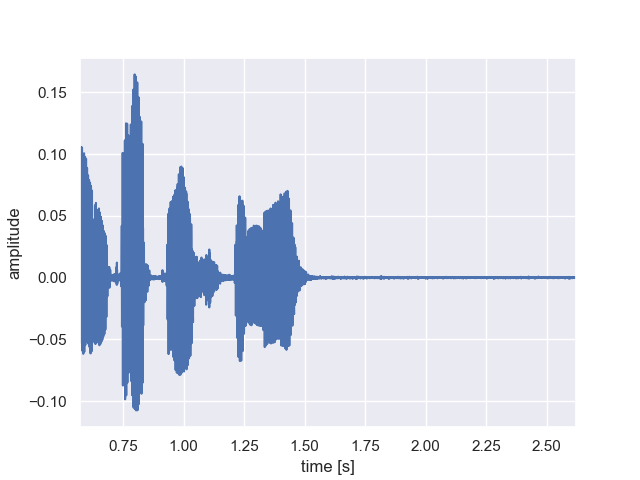
\includegraphics[width=400px, height=150px]{sound.png}%%
\caption{Wave-Form Plot}%%
\end{figure}

%
\subsection{Spectrogram of selected part of the audio signal}%
\label{subsec:Spectrogramofselectedpartoftheaudiosignal}%
\begin{figure}[h!]%%
\centering%%
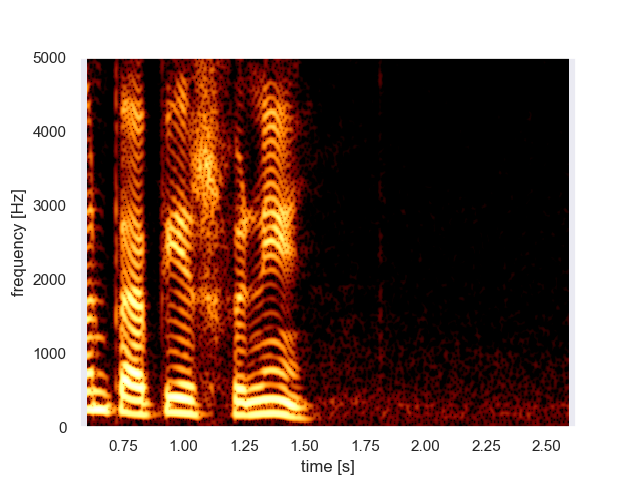
\includegraphics[width=400px, height=150px]{spectrogram.png}%%
\caption{Spectrogram Plot}%%
\end{figure}

%
\pagebreak[4]

%
\section{Pitch Analysis on the selected part}%
\label{sec:PitchAnalysisontheselectedpart}%


\begin{figure}[h!]%
\centering%
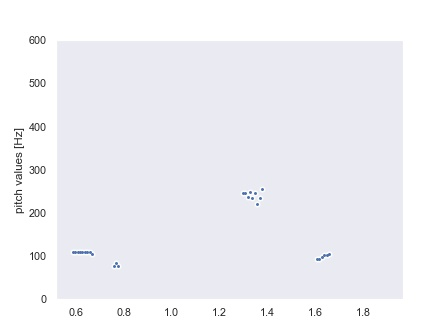
\includegraphics[width=300px]{pitch.jpg}%
\caption{Pitch Plot}%
\end{figure}

%
\subsection{Pitch}%
\label{subsec:Pitch}%
Mean value : 202.4789071234105%
\newline%
Median value : 62.85210090588376

%
\subsection{Subject Gender prediction based on pitch analysis}%
\label{subsec:SubjectGenderpredictionbasedonpitchanalysis}%
Predicted Gender of the Subject is {[}'male'{]}

%
\pagebreak[4]

%
\section{Formant Analysis on the selected part}%
\label{sec:FormantAnalysisontheselectedpart}%


\begin{figure}[h!]%
\centering%
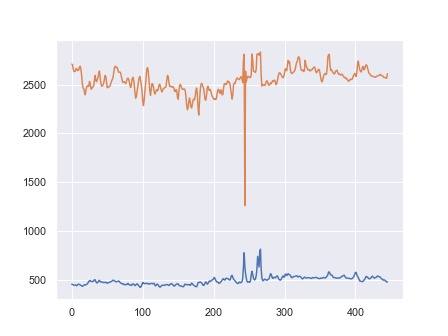
\includegraphics[width=300px]{formant.jpg}%
\caption{Formant Plot}%
\end{figure}

%
\subsection{First Formant}%
\label{subsec:FirstFormant}%
Mean value : 473.27821331402623%
\newline%
Median value : 389.35128966113496

%
\subsection{Second Formant}%
\label{subsec:SecondFormant}%
Mean value : 1814.5159691731599%
\newline%
Median value : 1829.3946291413836

%
\end{document}